\documentclass[12pt]{article}
\usepackage{blindtext}
\usepackage{hyperref}
\usepackage[total={7in, 9in}]{geometry}
\usepackage[utf8]{inputenc}
\usepackage{graphicx}
\usepackage{amsmath}
\usepackage{amsfonts}
\usepackage{amssymb}

% Title Page
\title{E102 Final Report}
\author{Pierce Gruber, Kaitlin Lucio}


\begin{document}
\maketitle

\begin{abstract}
Moving a cart with an inverted pendulum is an inherently tricky system as it requires both disturbing and maintaining an unstable equilibrium to move the cart to a desired location. This report describes a solution for such a system obtained via pole placement MATLAB Simulink.
\end{abstract}

\section{Problem Statement}
A cart with an inverted pendulum of length $L = 0.5\text{ m}$ and a max acceleration of $|\text{a}(t)| < 0.5 \text{ m}/\text{sec}^2$ and is subject to an angular acceleration disturbance $\alpha(t) = 0.5$ rad$/\text{sec}^{2}$. The cart must move to a final displacement from its starting location of $10$ m within an overall time limit of $10$ seconds without overshooting its target. The cart is able to measure its displacement $s(t)$ and its current pendulum angle $\theta(t)$. A diagram of the problem is given below

\begin{center}
    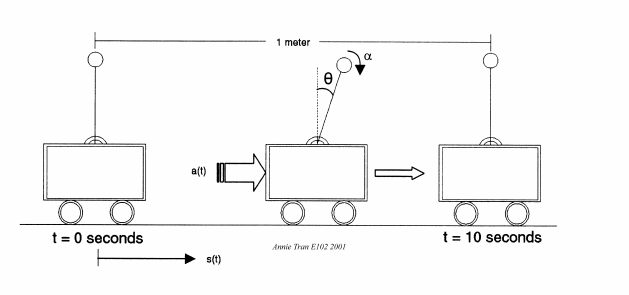
\includegraphics{graphs/invpen.png}
\end{center}
\newpage
The governing equations for this system are given by the following

\begin{align*}
    L\frac{d^{2}\theta}{dt^{2}} &- g\text{sin}(\theta(t)) = -a(t)\text{cos}(\theta(t)) + L\alpha(t) \\
    \frac{d^2s}{dt^2} &= a(t)
\end{align*}

Rearranging yields the following governing equations

\begin{align*}
    \frac{d^{2}\theta}{dt^{2}} &= \frac{g}{L}\text{sin}(\theta(t)) - \frac{1}{L}a(t)\text{cos}(\theta(t)) + \alpha(t) \\
    \frac{d^2s}{dt^2} &= a(t)
\end{align*}

and for a state-space set of equations, these equations must be linear. Using $\text{sin}(\theta) = \theta$ and $\text{cos}(\theta) = 1$ to linearize the equations results in

\begin{align*}
    \frac{d^{2}\theta}{dt^{2}} &= \frac{g}{L}\theta - \frac{1}{L}a(t) + \alpha(t) \\
    \frac{d^2s}{dt^2} &= a(t)
\end{align*}

Given state vector $\bar{x} = \begin{bmatrix} \theta \\ \dot{\theta} \\ s \\ \dot{s} \end{bmatrix}$ and control input $u = a(t)$, a disturbance $\omega = \alpha(t)$, and an output vector $\bar{y} = \begin{bmatrix} \theta \\ s \end{bmatrix}$, we can write out a set of matrices for this system when not in any sort of feedback. This results in the following matrices for the state space equations $\dot{\bar{x}} = A\bar{x} + Bu$ and $\bar{y} = C\bar{x} + Du$.

\begin{center}
    \begin{tabular}{| c | c | c | c |}
        \hline
        A & B & C & D \\
        \hline
        $\begin{bmatrix}
                0 & 1 & 0 & 0 \\
                \frac{g}{L} & 0 & 0 & 0 \\
                0 & 0 & 0 & 1 \\
                0 & 0 & 0 & 0
             \end{bmatrix}$
        &
        $\begin{bmatrix}
                0 \\ -\frac{1}{L} \\ 0 \\ 1
             \end{bmatrix}$
        &
        $\begin{bmatrix}
                1 & 0 & 0 & 0 \\
                0 & 0 & 1 & 0
             \end{bmatrix}$
        &
        $\begin{bmatrix}
                0 \\ 0
             \end{bmatrix}$ \\
        \hline
    \end{tabular}
\end{center}

where we ignore the disturbance $\alpha(t)$.

We note that for our system as described above, we can calculate $M_c$ and $M_o$. This results in the following matrices.

\begin{center}
    \begin{tabular}{| c | c |}
        \hline
        $M_c$ & $M_o$ \\
        \hline
        $\begin{bmatrix}
            0 & -2 & 0 & -39.2 \\
            -2 & 0 & -39.2 & 0 \\
            0 & 1 & 0 & 0 \\
            1 & 0 & 0 & 0
        \end{bmatrix}$
        &
        $\begin{bmatrix}
            1 & 0 & 0 & 0 \\
            0 & 0 & 1 & 0 \\
            0 & 1 & 0 & 0 \\
            0 & 0 & 0 & 1
        \end{bmatrix}$ \\
        \hline
    \end{tabular}
\end{center}

which are both invertible and thus the system is both invertible and controllable.

In addition, we created a Simulink model for simulation with saturation. This is pictured along with any MATLAB code in the Appendix.

\section{State Space Design for Linear System}

Now we will design a controller in feedback to tune the poles of the system to have the desired response characteristics. We will also design an observer to estimate the state of the system quickly and implement integral action to deal with the disturbance and ensure 0 steady state error without overshoot.

Since our input is 1D and our state is 4D, we will have a fifth order system. To make designing the poles easier, we can place two of the poles to be dominant to make the system behave like 2nd order. The other three poles could then be placed to be much faster than the dominant poles so as to not contribute to the system dynamics.

To find where to place the dominant poles to satisfy the desired response characteristics, we can assume $\zeta \ge 1$ to allow for no overshooting. To find a starting point for $\omega_n$, we can solve the critically damped general equation for a unit step input and settling time (within 99\%) of 10 seconds:

\begin{align*}
    x(t_s) &= 0.99 = \frac{1}{\omega_n^2}(1-e^{-\omega_nt_s} - \omega_nt_se^{-\omega_nt_s}) \\
    t_s &= 8
\end{align*}

Plugging this into Wolfram Alpha, $\omega_n \approx 1$. This was the starting point for the poles to be tuned. A MATLAB script was then written to find the roots of the characteristic polynomial, the dominant poles, given $\zeta$ and $\omega_n$. The non-dominant poles were then placed to be ten times faster than the dominant poles.

Now that we have poles, we need to calculate the feedback matrices for an integral action system so that we can use the place command. Note that since our integral action only acts on one output, we only use the row from $C$ which is multiplied by $s$. This results in the following matrices

\begin{center}
    \begin{tabular}{| c | c | c | c |}
        \hline
        $A_{af}$ & $B_{af}$ & $C_{af}$ & $D_{af}$ \\
        \hline
        $\begin{bmatrix}
                0 & 0 & 0 & -1 & 0 \\
                0 & 0 & 1 & 0 & 0 \\
                0 & \frac{g}{L} & 0 & 0 & 0 \\
                0 & 0 & 0 & 1 & 0 \\
                0 & 0 & 0 & 0 & 0
        \end{bmatrix}$
        &
        $\begin{bmatrix}
                0 \\ 0 \\ -\frac{1}{L} \\ 0 \\ 1
        \end{bmatrix}$
        &
        $\begin{bmatrix}
                0 & 0 & 0 & 1 & 0
        \end{bmatrix}$
        &
        $\begin{bmatrix}
                0 \\ 0
        \end{bmatrix}$ \\
        \hline
    \end{tabular}
\end{center}

\section{Simulation of Nonlinear System using Linear Controller}

Beginning with no disturbance and starting at the values $\zeta = 1$ and $\omega_n = 1$, we ran the simulation of the complete system and found it to be unexpectedly unstable despite all closed loop poles being negative and real valued. We realized that our observer poles were too slow, and after increasing their speed, the system became stable. Once the disturbance was taken into account though, $\zeta$, $\omega_n$, and the observer pole speed needed to be tuned again to keep the system stable. Specifically, the observer poles needed to be faster, and thus were set to 50 times the speed of the dominant poles in the feedback controller.

Initial attempts to increase $\zeta$ to 1.2 and decrease $\omega_n$ to 0.48 did not meet constraints, being stable at a maximum disturbance of only 0.2. By analyzing input acceleration over time and comparing the bounded value to the system's desired values, we were able to figure out slightly better values around $\zeta = 1.01$ and $\omega_n = 0.6$.

By performing a parameter sweep of $\zeta$ and $\omega_n$ above but near the aforementioned better values and then analyzing the results in terms of overshoot and settling time, we obtained the parameters $\zeta = 1.005$ and $\omega_n = 0.7$, which yielded a settling time of 8.46 s and a maximum disturbance $0.707 \text{rad}/\text{s}^{2}$. The plots of both specification disturbance $0.5$ and the maximum disturbance can be found below along with the respective $K$, $K_I$, and $L$ matrices for this system.

\begin{center}
    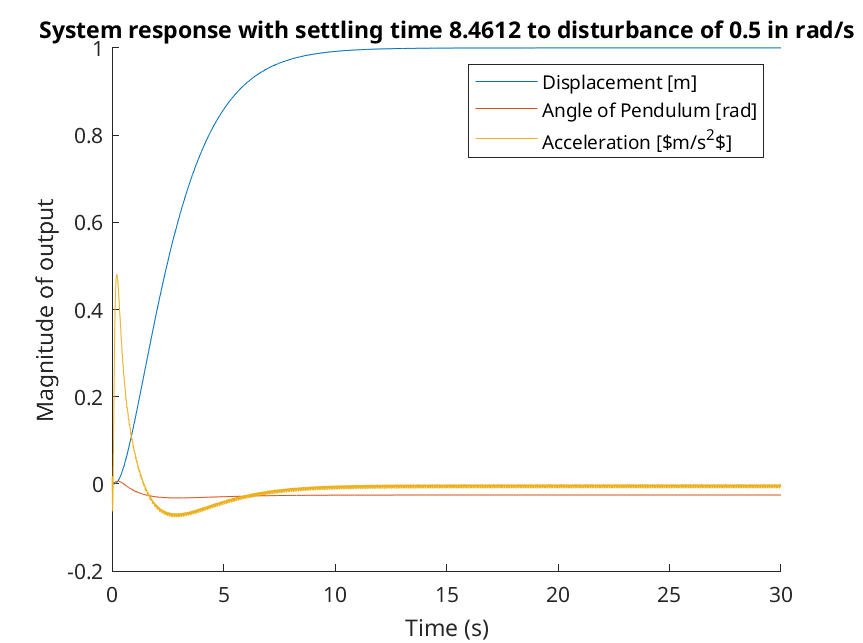
\includegraphics[width=3in]{graphs/sim_displacement_0.5.png}
    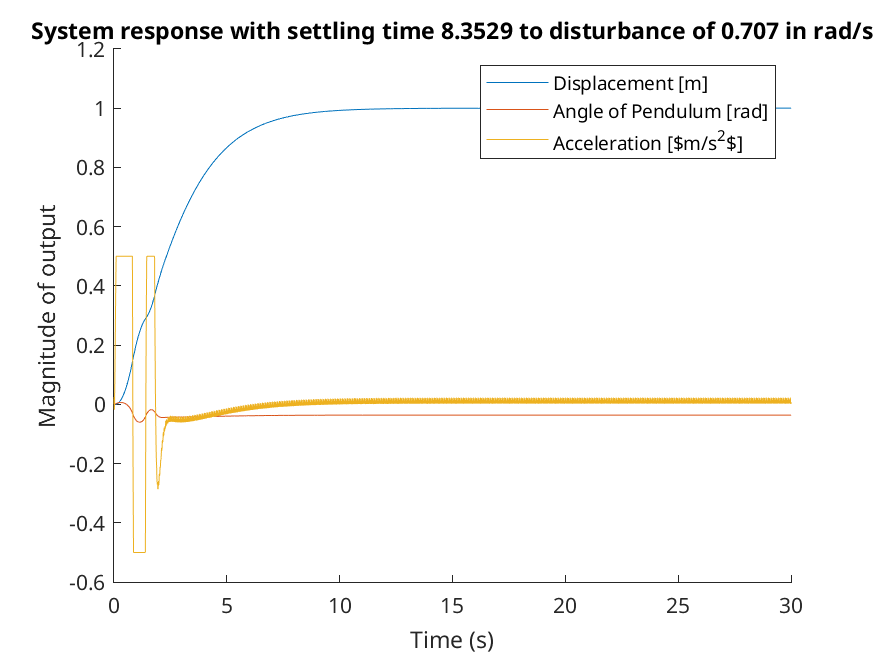
\includegraphics[width=3in]{graphs/sim_displacement_0.707.png}
\end{center}


\begin{center}
    \begin{tabular}{| c | c | c |}
        \hline
        $K$ & $K_I$ & $L$ \\
        \hline
        $\begin{bmatrix}
            -153.5345 & -35.6838 & -45.8294 & -45.0510
        \end{bmatrix}$
        &
        $\begin{bmatrix}
            14.1661
        \end{bmatrix}$
        &
        $\begin{bmatrix}
            418.606201507400 & 2.89061140408423 \\
            12307.8691984876 & 434.197695377039 \\
            2.67046905825809 & 502.689988411429 \\
            379.624655238968 & 17910.6286611251
        \end{bmatrix}$ \\
        \hline
    \end{tabular}
\end{center}
\section{Results and Conclusion}

The system described above is able to handle a disturbance of up to $\alpha = 0.707 \text{rad}/\text{s}^{2}$ while also settling at the final position well ahead of the actual constraint of $10$ seconds. This may not be the most optimal system, as another set of parameters may be able to trade a little bit of the settling speed for more stability and thus that system would be able to handle a larger angular disturbance to the system. This is more than findable with a little bit more testing and coding.

As discussed previously, the saturation limit on the acceleration is difficult to work around as many combinations of $\zeta$ and $\omega_n$ which would be stable without saturation become unstable as the system is unable to correct itself from an otherwise recoverable state. As such, trial and error and parameter sweeps were crucial in designing a functioning system.

\newpage

\section{Appendix}

\subsection{Code Repository}

MATLAB code can be found on our \href{https://github.com/slmnemo/e102invpend}{Github Repository here}. Important functions have been pasted at the very end.

\subsection{Simulink Blocks}

\begin{center}
    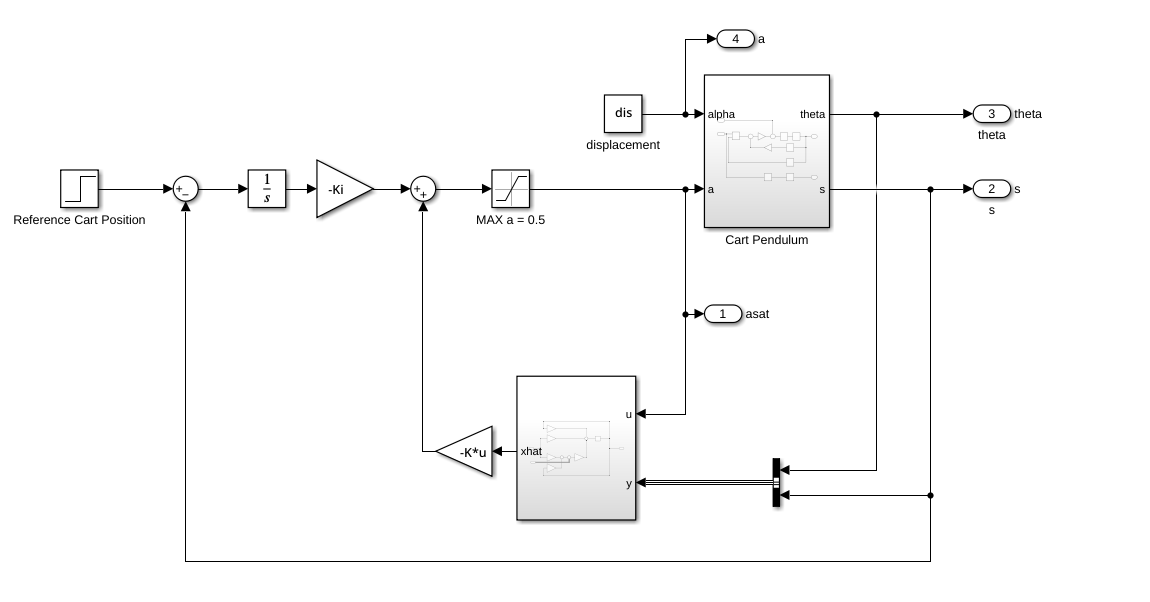
\includegraphics[width=6in]{graphs/simulinkfull.png} \\
    Image of full Simulink
\end{center}

\begin{center}
    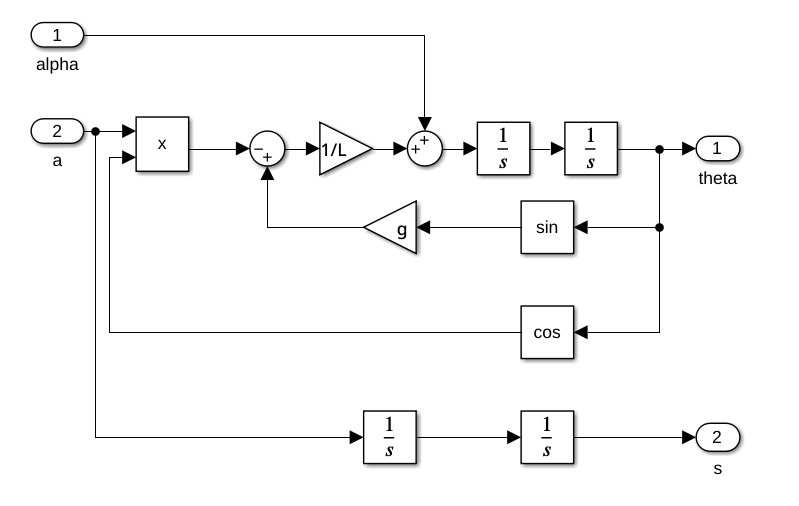
\includegraphics[width=6in]{graphs/simulinkcontroller.png} \\
    Image of controller subblock inside larger model
\end{center}

\begin{center}
    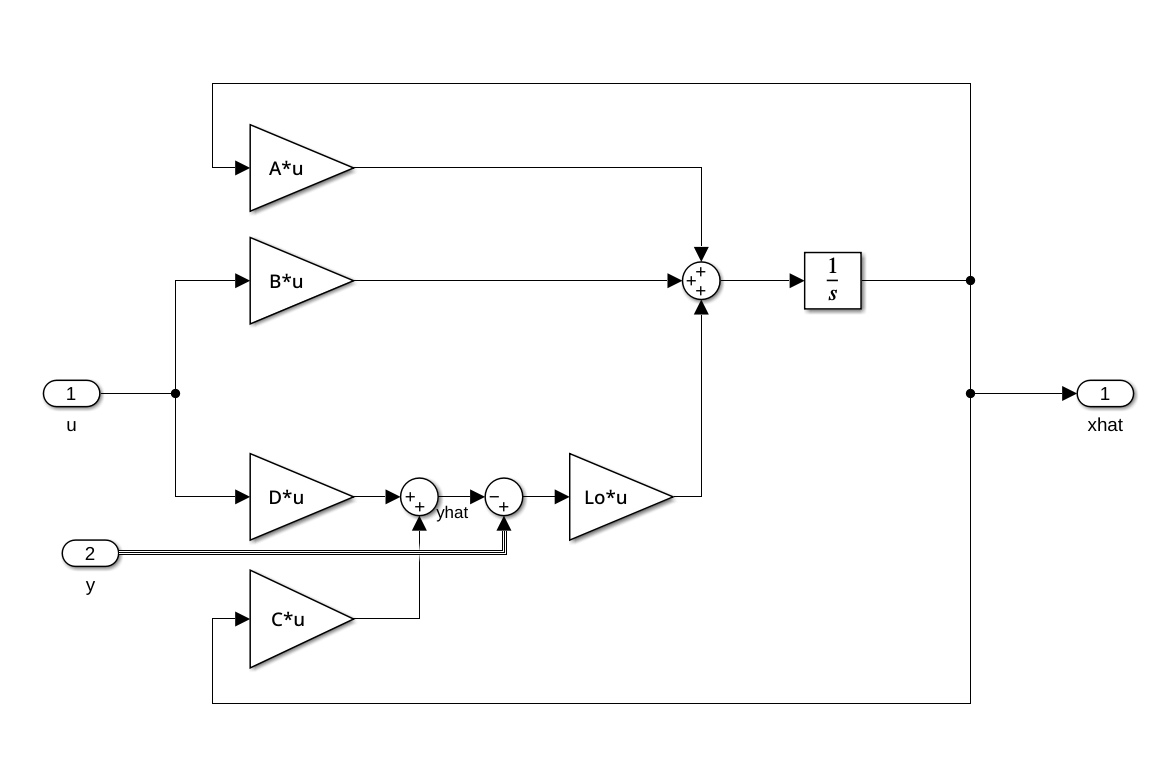
\includegraphics[width=6in]{graphs/simulinkobserver.png} \\
    Image of observer subblock inside larger model.
\end{center}

\newpage

\subsection{Raw MATLAB code}

\begin{verbatim}
main.m

% Written by Pierce Gruber and Kaitlin Lucio
clear
clf

% Variable definitions
zeta = 1.005;
wn = 0.7;
testmode = false;
dis_start = 0.5;
dis_step = 0.001;
dis_stop = 0.7;
dis = dis_start;
distvec = dis_start:dis_step:dis_stop;


% Pole modifiers
conPmod = 10;
obsPmod = 50;
KiPmod = 10.2;

% Simulate Simulink model
if testmode
    sim_run = sim("plant.mdl");
    plot(sim_run.yout)
else
    i = 1;

    figurefolder = "figures/";
    figprefix = "sim_displacement_";

    for dim=distvec
        dis = dim;
        [os, t_settle, sim_run] = sim_invpendulum(dis,zeta,wn,conPmod,obsPmod,KiPmod);
        s = sim_run.yout{2}.Values.Data;
        theta = sim_run.yout{3}.Values.Data;
        a = sim_run.yout{1}.Values.Data;
        time = sim_run.tout;
        figure(i)
        hold on
        plot(time, s)
        plot(time, theta)
        plot(time, a)
        xlabel("Time (s)")
        ylabel("Magnitude of output")
        legend("Displacement [m]", "Angle of Pendulum [rad]", "Acceleration [$m
        /s^2$]")
        title("System response with settling time "+num2str(t_settle)+" to
        disturbance of "+num2str(dis)+" in rad/s")
        saveas(i,figurefolder+figprefix+num2str(dis)+".png")
        close(i)
        i = i + 1;
    end
end
\end{verbatim}

\newpage

\begin{verbatim}
sim_invpendulum.m

function [overshoot, t_settle, sim_data] = sim_invpendulum(ang_dis, zeta, wn,
conPmod, obsPmod, KiPmod, p)
%{
    Function to simulate a 5th order inverted pendulum using pole
    placement. Takes in a zeta and omega measurement and returns the
    overshoot and settling time.

    Zeta must be >= 1

    Omega must be > 0

    dis is a disurbance in angular momentum applied at t = 0.

    Written by Pierce Gruber and Kaitlin Lucio
%}

% Variable definitions

L = 0.5;
g = 9.8;

% Define A, B, C, and D

A = [
    0, 1, 0, 0;
    g/L, 0, 0, 0;
    0, 0, 0, 1;
    0, 0, 0, 0
];

B = [0; -1/L; 0; 1];

C = [
    1, 0, 0, 0;
    0, 0, 1, 0
    ];

D = [
    0;
    0
    ];

% Pole calculations
% 2nd order dominant system
domPolynom = [1 2*zeta*wn wn^2];
domPoles = roots(domPolynom);
conPoles = [domPoles' min(domPoles)*conPmod min(domPoles)*1.2*(conPmod)];

% The observer poles are just the controller poles but made to be
% faster.
obsPoles = obsPmod*conPoles;
Lo = place(A', C', obsPoles)';

% Calculate Ki_fb and K_fb using integral action state matrices

% Add the fifth pole, the integral control pole.
KiPole = domPoles(1)*KiPmod;
allPoles = [conPoles KiPole];

% Define full integral action poles and calculate Ki and K.

Aa = [
    0, -C(2,:);
    zeros(4,1), A
    ];
Ba = [
    -D(2); B
];

Ktot = acker(Aa, Ba, allPoles);
Ki = Ktot(1);
K = Ktot(2:end);

% Calculate Observer using poles from above

Lo = place(A', C', obsPoles)';

% Simulate Simulink model and get stats
dis = ang_dis;
h = load_system("plant.mdl");
hws = get_param(bdroot,'modelworkspace');
hws.assignin('dis',dis)
hws = get_param('plant','modelworkspace');
list = whos;
N = length(list);
for i = 1:N
    hws.assignin(list(i).name,eval(list(i).name))
end
sim_data = sim("plant.mdl");
info = stepinfo(sim_data.yout{2}.Values.Data,sim_data.tout,"SettlingTimeThreshold",0.02);
overshoot = info.Overshoot;
t_settle = info.SettlingTime;
\end{verbatim}

\newpage

\begin{verbatim}
search_invpen.m

%{
    Wrapper file to find good poles for an inverted pendulum
%}

zetarange = 1.005:0.001:1.015;
wrange = 0.5:0.01:0.7;
conPmodrange = 10:2:10;
obsPmodrange = 50:5:50;
KiPmodrange = 10.3:0.2:10.3;
dis = 0.5;
t_settle_thres = 10;
os_thres = 1;

outcsv = "figures/invpen_vals_disp"+num2str(dis)+".csv";
file = fopen(outcsv,"w");
fprintf(file, "idx, zeta, omega, t_set,conPmod,obsPmod,KiPmod\n");
fspec = "%d, %2.4f, %2.4f, %2.4f, %2.1f, %2.1f, %2.1f\n";

k = 0;
for zetaCon = zetarange
    for wCon = wrange
        for conPmod = conPmodrange
            for obsPmod = obsPmodrange
                for KiPmod = KiPmodrange
                    [os, t_settle, sys_data] =
                    sim_invpendulum(dis,zetaCon,wCon,conPmod,obsPmod,KiPmod);
                    fprintf("testing %.4f, %.4f, %2f, %2f,
                    %2f\n",zetaCon,wCon,conPmod,obsPmod,KiPmod);
                    if (os < os_thres) && (t_settle < t_settle_thres)
                        fprintf(file, fspec, k, zetaCon, wCon, t_settle, conPmod,
                        obsPmod, KiPmod);
                        k = k + 1;
                    end
                end
            end
        end
    end
end

file = fclose(file);
\end{verbatim}

\newpage

\begin{verbatim}
testObservability.m

function [Mo, invMo] = testObservability(A, C)
%{
    Takes in a state-space matrix A and C and displays whether the observer
    matrix is invertible, and thus if the system is observable. Errors if
    unobservable.
%}

[Mo, invMo] = MO_calc(A, C);

if det(Mo) == 0
    error("Not Observable! Mo is not invertible [determinant = 0]")
else
    disp("Mo is invertible, this system is observable!")
end
\end{verbatim}

\newpage

\begin{verbatim}
testControllability.m

function [Mc, invMc] = testControllability(A, B)
%{
    Takes in a state-space matrix A and B and displays whether the control
    matrix is invertible, and thus if the system is controllable. Errors if
    uncontrollable.
%}

[Mc, invMc] = MC_calc(A, B);

if det(Mc) == 0
    error("Mo is not invertible [determinant = 0]")
else
    disp("Mo is invertible, this system is controllable!")
end
\end{verbatim}

\end{document}
